%% Autor: Björn Ritterbecks 
%% Letzte Aenderung: 15.06.2016 
\thisfloatsetup{%
  capbesidewidth=\marginparwidth,}
\begin{figure}[htbp]
\centering
%\sansmath
\begin{tikzpicture}[      
        every node/.style={anchor=south west,inner sep=0pt},
        x=1mm, y=1mm,
      ]   
     \node (fig1) at (0,0)
       {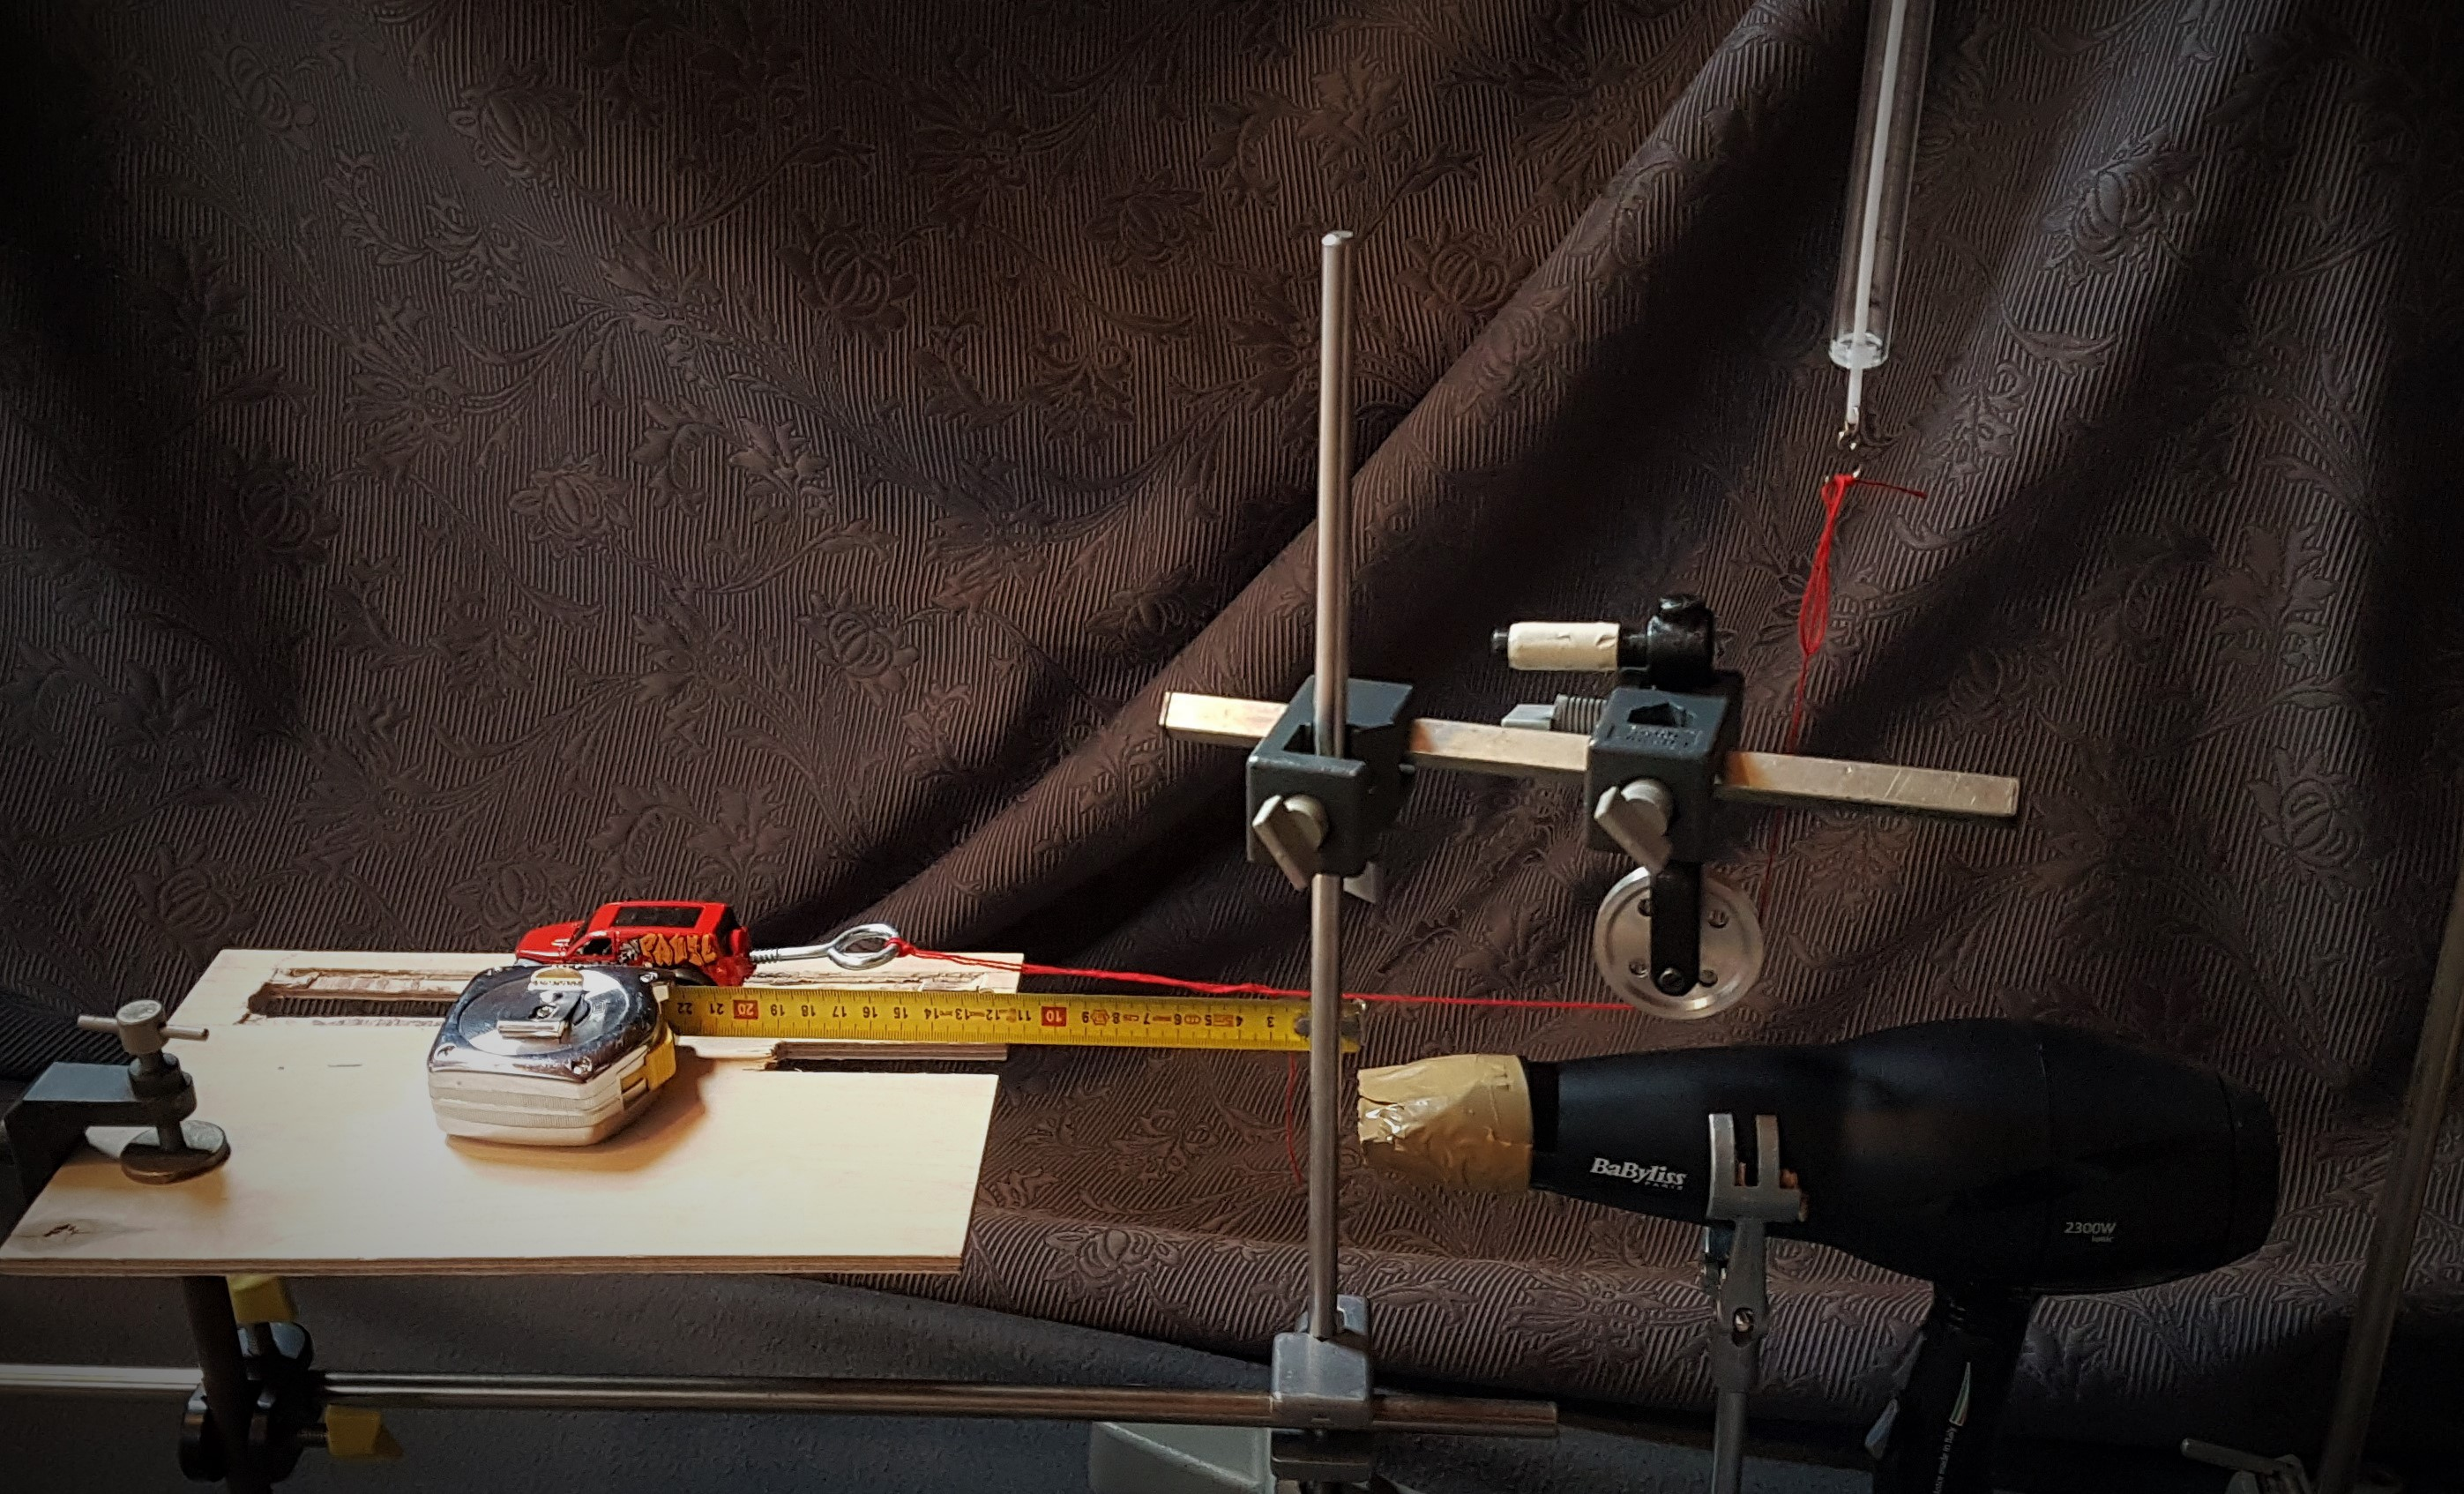
\includegraphics[scale=0.108]{images/stroemungskraftmessung1.jpg}};
     \node (fig2) at (3,40)
       {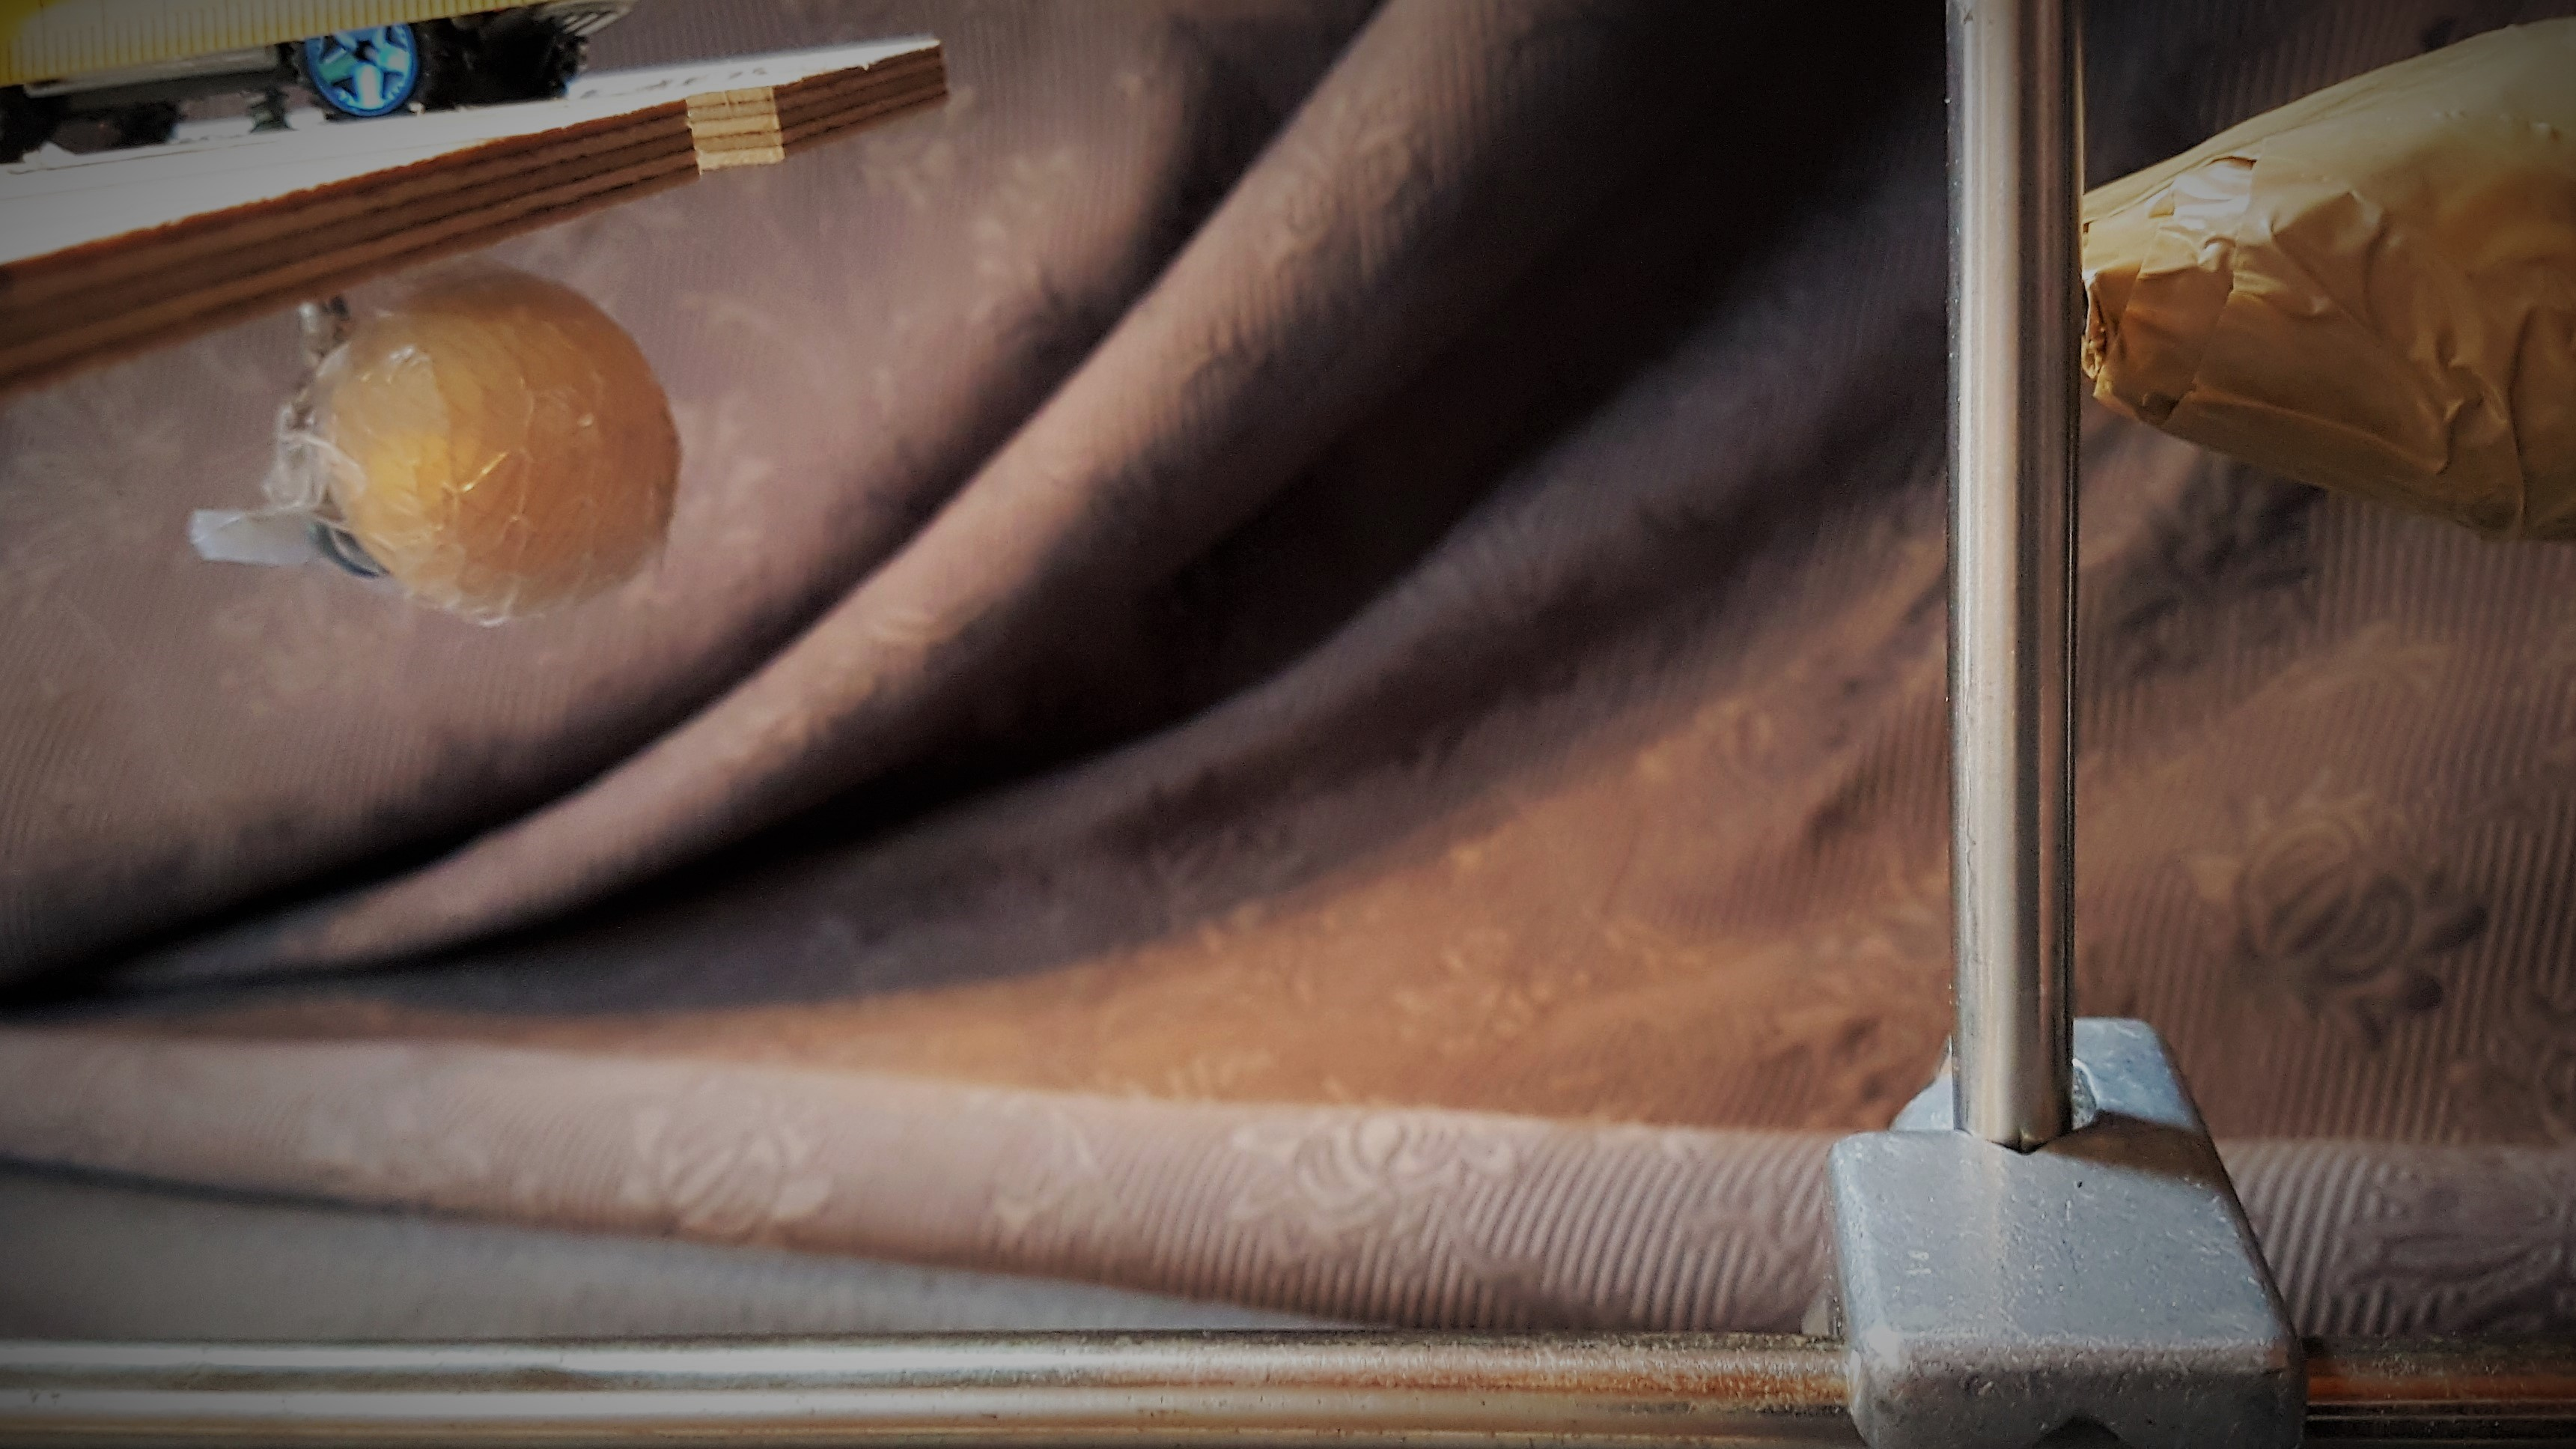
\includegraphics[scale=0.027]{images/stroemungskraftmessung2.jpg}};  
\end{tikzpicture}
  \caption[Erster Versuchsaufbau zur Strömungskraftmessung]{Erster Versuchsaufbau zur Strömungskraftmessung: Ein Messwagen, an dem eine Kugel aufgehängt wird, ist mit einem Federkraftmesser über eine Umlenkrolle verbunden. Die Unterseite der Messplatte ist als Auszug links oben im Foto abgebildet.}
  \label{fig:stroemungskraftmessung1}
  \vspace{-0pt}
\end{figure}